\documentclass[11pt,a4paper]{mwart}
\usepackage[english,polish]{babel}
\usepackage[T1]{fontenc}
\usepackage[UTF8]{inputenc}
\usepackage{polski}
\usepackage{amsmath}
\usepackage{euler}
\usepackage{plain}
\usepackage{graphicx}
\usepackage{tikz}
\title{Aplikacja dla dyspozytora}
\author{Andrzej Samson, Jędrzej Wiśniewski}
\date{\today}

\begin {document}
\maketitle
\section{Zadanie} 
Celem zadania jest stworzenie aplikacji dla dyspozytora, w której będzie można przydzielać zlecenia do samochodów w firmie. W aplikacji możliwe będzie zobaczenie miejsca, w którym znajduje się kierowca, do jakiego punktu zmierza, ile mu to zajmie czasu oraz masa jego ładunku. Dyspozytor z poziomu aplikacji będzie miał możliwość przerwania podróży samochodu i wysłanie go natychmiastowo do bazy. Aplikacja będzie uwzględniać czas jaki należy pokonać między kolejnymi punktami. Odległości między punktami będą podawane w czasie, jaki samochód potrzebuje, aby pokonać dany odcinek drogi. Ładowność samochodu podawana będzie w kilogramach. Odległości między punktami będą stałe. Czas załadunku i rozładunku to 30 minut.
\subsection{Problem komiwojażera}
Problem polega na optymalizacji trasy, czyli znalezieniu trasy do podróży w taki sposób, aby każdy punkt tej trasy odwiedzić tylko raz i to jak najbardziej optymalnie, czyli np. żeby koszt był jak najmniejszy lub podróż trwała jak najkrócej. Problem ten zalicza się do NP-trudnych, czyli takich, gdzie ciężko jest znaleźć algorytm rozwiązujący ten problem, który jest najbardziej optymalny i najlepszy. Dlatego często rozwiązuje się takie problemy, znajdując rozwiązanie przybliżone do tego najbardziej optymalnego.
\section{Specyfikacja}
Nasza firma dostawcza oraz główna baza znajdują się w Łodzi. Stąd będą rozpoczynać trasę wszystkie samochody i załatwiać przypisane im zlecenia. Jest to też miejsce do którego muszą wrócić gdy dyspozytor wyda im polecenie powrotu. 
\subsection{Samochody i towar}
Firma ma do dyspozycji \textit{N} samochodów dostawczych, każdy o ładowności 1000 kg. Aby samochód wyruszył z bazy nie musi być w pełni załadowany, gdyż celem jest jak najbardziej optymalna realizacja zleceń. Dopuszczalny jest również tzw. pusty przebieg, czyli podróż bez towaru do jakiegoś punktu (miejscowości), aby wypełnić zlecenie lub w przypadku powrotu do bazy, gdy dyspozytor wyda polecenie powrotu bezpośredniego. Samochód nie może wziąć takiej liczby towarów, która przekroczyłaby jego ładowność. 
\subsection{Miejscowości i trasa}
Na \textit{rysunku 1} przedstawiona została mapa Polski na której zaznaczone są miejscowości do których podróżują samochody firmowe, punkty łączące dane odcinki oraz trasy między nimi jakie mają do pokonania. Wszystkie zaznaczone odcinki posiadają przypisany numer oraz czas podróży między dwoma punktami. W celu znalezienia najbardziej optymalnej trasy, aplikacja będzie znajdować wszystkie możliwe drogi, aby dotrzeć do punktu końcowego, sumować czas jaki należy pokonać między danymi odcinkami, porównywać je między sobą, a następnie wyświetlać najszybsze trasy podróży. Dla firmy najważniejszym celem jest jak najszybsze wypełnienie zlecenia.
\begin{figure}[th]
\centering
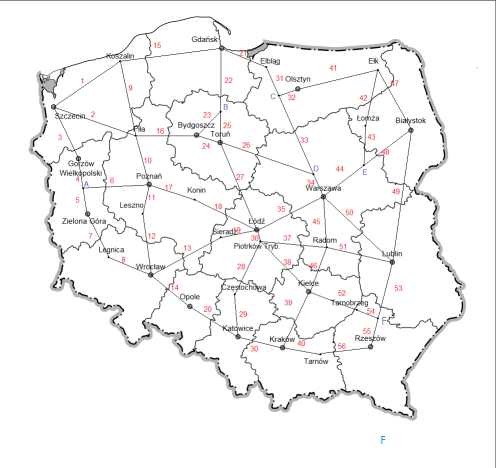
\includegraphics[width=\textwidth]{mapa.png}
\caption{Mapa miejscowości i tras razem z numeracja}
\end{figure}

\section{Algorytm}
W naszej aplikacji będziemy używać algorytmu Dijkstry. Służy on do wyznaczania najmniejszej odległości od ustalonego punktu do wszystkich pozostałych, ustalonych w grafie. W algorytmie tym pamiętany jest zbiór Q wierzchołków, dla których nie obliczono jeszcze najkrótszych ścieżek, oraz wektor D[i] odległości od wierzchołka początkowego do \textit{i}. Algorytm przebiega następująco:
\begin{flushleft}
\begin{enumerate}
\item[a]. Dopóki zbiór Q nie jest pusty wykonuj:
\item[b]. Pobierz ze zbioru Q wierzchołek \textit{v} o najmniejszej wartości D[v] i usuń go ze zbioru.
\item[c]. Dla każdego następnika \textit{i} wierzchołka v dokonaj relaksacji ścieżki, tzn. sprawdź, czy D[i]>D[v]+A[v,i], tzn czy aktualne oszacowanie odległości do wierzchołka \textit{i} jest większe od oszacowania odległości do wierzchołka \textit{v} plus waga krawędzi (v,i).
Jeżeli tak jest, to zaktualizuj oszacowanie D[i] przypisując mu prawą stronę nierówności (czyli mniejszą wartość).\\
\end{enumerate}
\end{flushleft}
Z algorytmu Dijkstry można skorzystać przy obliczaniu najkrótszej drogi do danej miejscowości. Wystarczy przyjąć, że każdy z punktów skrzyżowań dróg to jeden z wierzchołków grafu, a odległości między punktami to wagi krawędzi.
\section{Baza danych}
Aplikacja będzie korzystać z baz danych SQL-owych. Skrypt do naszej bazy jest zapisany za pomocą SQlite.
Z bazy danych aplikacja będzie otrzymywać informacje o:
\begin{enumerate}
\item[• Samochody]
\item[• Wierzchołki mapy]
\item[• Zlecenia]
\item[• Wykonanie zleceń]
\end{enumerate}
\section{Dyspozytor i interfejs}
Dyspozytor jest \textbf{użytkownikiem} aplikacji. Może on poprzez aplikacje tworzyć nowe zlecenia - przydzielać masę towaru jaka ma być z danej miejscowości pobrana oraz do której miejscowości ją zawieźć. Dyspozytor przydziela samochody do zlecenia. Może też zawrócić samochód do bazy. Jeżeli po komendzie powrotu samochód jest pusty to wykonuje on pusty przebieg. 
Poprzez interfejs dyspozytor ma dostęp do:
\begin{flushleft}
\begin{enumerate}
\item[• Zlecenia] - dodawanie nowych zleceń, przydzielanie istniejących zleceń do kierowców oraz przegląd zakończonych już zleceń - daty przyjścia i zakończenia, jaki kierowca wykonywał zlecenie, masę oraz status zakończenia.
\item[• Samochody] - wgląd do opisu samochodu, czyli na jakiej trasie jest samochód, jakie wykonuje zlecenie i ile czasu pozostało mu do zakończenia zlecenia. W tym miejscu będzie również możliwość odesłania samochodu bezpośrednio z powrotem do bazy.
\item[• Opcje] - opcje aplikacji, opis korzystania z aplikacji oraz zamknięcie programu
\end{enumerate}
\end{flushleft}
Aplikacja została stworzona w języku python oraz przy pomocy pakietu wx.Python w celu stworzenia interfejsu. Aby można było przeprowadzać testu i sprawdzać jej działanie, odległości między miejscowościami przedstawione zostały w sekundach a nie minutach. W ten sposób można łatwiej kontrolować, czy wszystko działa. Aplikacja odświeża się co 5 sekund, porównując w tym czasie czas aktualny z czasem jaki został kierowcom do końca zlecenia. jeżeli czas aktualny przekroczy czas zakończenia zlecenia, wtedy automatycznie odświeżają się baza danych. Aktualizowane są zlecenia, miejsce przebywania kierowcy oraz zakończenie zleceń. W opcjach można uzyskać informacje o działaniu każdej funkcji aplikacji.
\end {document}